\documentclass[11pt]{article}


% Page size
\usepackage[top=1.2in, bottom=1.2in, left=1.4in, right=1.4in]{geometry}

% Load Packages --------
\usepackage{placeins}
\usepackage{graphicx,grffile}

%% Math ----
\usepackage{amssymb, amsmath, amsthm}

%% Tables ---


% Fonts ---------

% Color
\usepackage{xcolor}
\definecolor{crimson}{RGB}{156,0,0}


%% Implement textsf for everything
\usepackage[sfdefault]{roboto}
\renewcommand{\familydefault}{\sfdefault}
\usepackage[cm]{sfmath}

%% Hyperref
\usepackage[hidelinks = true,
            colorlinks = true,
            urlcolor = crimson,
            linkcolor = crimson]{hyperref}


% Tight list ---

\providecommand{\tightlist}{%
  \setlength{\itemsep}{0pt}\setlength{\parskip}{0pt}}

% Math commands --------

\newcommand{\var}{\textnormal{Var}}
\newcommand{\cov}{\textnormal{Cov}}
\newcommand{\cor}{\textnormal{Cor}}

% Highlighters

% code
\usepackage{xcolor}
\definecolor{light-gray}{gray}{0.95}
\newcommand{\code}[1]{\colorbox{light-gray}{\texttt{#1}}}
\newcommand{\highlight}[1]{\colorbox{yellow}{#1}}

% foots
\usepackage[hang, bottom]{footmisc}
\setlength{\footnotemargin}{1.2em} % separation between number and text
\interfootnotelinepenalty=10000 %% Completely prevent breaking of footnotes

% Figure caption?
\usepackage[labelfont=bf]{caption}
\setlength{\captionmargin}{10pt}




% Actual Input ------
% Figures
\makeatletter
\def\maxwidth{\ifdim\Gin@nat@width>\linewidth\linewidth\else\Gin@nat@width\fi}
\def\maxheight{\ifdim\Gin@nat@height>\textheight\textheight\else\Gin@nat@height\fi}
\makeatother

% Scale images if necessary, so that they will not overflow the page
% margins by default, and it is still possible to overwrite the defaults
% using explicit options in \includegraphics[width, height, ...]{}
\setkeys{Gin}{width=\maxwidth,height=\maxheight,keepaspectratio}


% Shading and Rmd macros
\usepackage{color}
\usepackage{fancyvrb}
\newcommand{\VerbBar}{|}
\newcommand{\VERB}{\Verb[commandchars=\\\{\}]}
\DefineVerbatimEnvironment{Highlighting}{Verbatim}{commandchars=\\\{\}}
% Add ',fontsize=\small' for more characters per line
\usepackage{framed}
\definecolor{shadecolor}{RGB}{248,248,248}
\newenvironment{Shaded}{\begin{snugshade}}{\end{snugshade}}
\newcommand{\AlertTok}[1]{\textcolor[rgb]{0.94,0.16,0.16}{#1}}
\newcommand{\AnnotationTok}[1]{\textcolor[rgb]{0.56,0.35,0.01}{\textbf{\textit{#1}}}}
\newcommand{\AttributeTok}[1]{\textcolor[rgb]{0.77,0.63,0.00}{#1}}
\newcommand{\BaseNTok}[1]{\textcolor[rgb]{0.00,0.00,0.81}{#1}}
\newcommand{\BuiltInTok}[1]{#1}
\newcommand{\CharTok}[1]{\textcolor[rgb]{0.31,0.60,0.02}{#1}}
\newcommand{\CommentTok}[1]{\textcolor[rgb]{0.56,0.35,0.01}{\textit{#1}}}
\newcommand{\CommentVarTok}[1]{\textcolor[rgb]{0.56,0.35,0.01}{\textbf{\textit{#1}}}}
\newcommand{\ConstantTok}[1]{\textcolor[rgb]{0.00,0.00,0.00}{#1}}
\newcommand{\ControlFlowTok}[1]{\textcolor[rgb]{0.13,0.29,0.53}{\textbf{#1}}}
\newcommand{\DataTypeTok}[1]{\textcolor[rgb]{0.13,0.29,0.53}{#1}}
\newcommand{\DecValTok}[1]{\textcolor[rgb]{0.00,0.00,0.81}{#1}}
\newcommand{\DocumentationTok}[1]{\textcolor[rgb]{0.56,0.35,0.01}{\textbf{\textit{#1}}}}
\newcommand{\ErrorTok}[1]{\textcolor[rgb]{0.64,0.00,0.00}{\textbf{#1}}}
\newcommand{\ExtensionTok}[1]{#1}
\newcommand{\FloatTok}[1]{\textcolor[rgb]{0.00,0.00,0.81}{#1}}
\newcommand{\FunctionTok}[1]{\textcolor[rgb]{0.00,0.00,0.00}{#1}}
\newcommand{\ImportTok}[1]{#1}
\newcommand{\InformationTok}[1]{\textcolor[rgb]{0.56,0.35,0.01}{\textbf{\textit{#1}}}}
\newcommand{\KeywordTok}[1]{\textcolor[rgb]{0.13,0.29,0.53}{\textbf{#1}}}
\newcommand{\NormalTok}[1]{#1}
\newcommand{\OperatorTok}[1]{\textcolor[rgb]{0.81,0.36,0.00}{\textbf{#1}}}
\newcommand{\OtherTok}[1]{\textcolor[rgb]{0.56,0.35,0.01}{#1}}
\newcommand{\PreprocessorTok}[1]{\textcolor[rgb]{0.56,0.35,0.01}{\textit{#1}}}
\newcommand{\RegionMarkerTok}[1]{#1}
\newcommand{\SpecialCharTok}[1]{\textcolor[rgb]{0.00,0.00,0.00}{#1}}
\newcommand{\SpecialStringTok}[1]{\textcolor[rgb]{0.31,0.60,0.02}{#1}}
\newcommand{\StringTok}[1]{\textcolor[rgb]{0.31,0.60,0.02}{#1}}
\newcommand{\VariableTok}[1]{\textcolor[rgb]{0.00,0.00,0.00}{#1}}
\newcommand{\VerbatimStringTok}[1]{\textcolor[rgb]{0.31,0.60,0.02}{#1}}
\newcommand{\WarningTok}[1]{\textcolor[rgb]{0.56,0.35,0.01}{\textbf{\textit{#1}}}}


\title{ \LARGE\textbf{R Winter Assignment (Solutions)}}

\author{}


\date{Winter 2020, Pre-Assignment\footnote{This exercise was originally
  written by Shiro Kuriwaki and Dan Levy. Copyright: CC-BY.}}

\begin{document}

\maketitle

\begin{center}
\highlight{Due January 27, 2020}
\end{center}

\noindent Combined with the assigned primers, this set of exercises will
help you get you up and running with doing basic data analysis in R. The
Math Camp program will go over the exercise to clarify any points of
confusion.\footnote{That said, please feel free to contact Shiro (kuriwaki\@g.harvard.edu) if you have any questions in the meantime. }

\hypertarget{submission}{%
\subsection*{Submission}\label{submission}}
\addcontentsline{toc}{subsection}{Submission}

Do your work in the rstudio.cloud environment described below and submit
only the saved \texttt{.R} file to the Assignment Page which we will
announce we created. More details on how to do this are provided at the
beginning and end of this assignment.

\hypertarget{where-are-we-where-are-we-headed}{%
\subsection*{Where are we? Where are we
headed?}\label{where-are-we-where-are-we-headed}}
\addcontentsline{toc}{subsection}{Where are we? Where are we headed?}

Before you start this practice problem set, you should complete the
following RStudio Primers:

\begin{enumerate}
\def\labelenumi{\arabic{enumi}.}
\tightlist
\item
  \href{https://rstudio.cloud/learn/primers/1.1}{Visualization Basics}
\item
  \href{https://rstudio.cloud/learn/primers/1.2}{Programming Basics}
\item
  \href{https://rstudio.cloud/learn/primers/2.1}{Work with Tibbles}
\item
  \href{https://rstudio.cloud/learn/primers/2.2}{Isolating Data with
  dplyr}
\item
  \href{https://math-camp-2019.shinyapps.io/03a-deriving-mutate/}{Creating
  Variables and dataframes}
\end{enumerate}

\noindent If you are already familiar with R, you can just briefly
review these tutorials. After this assignment, we'll be offering several
more sessions to cover more tools and concepts.

\newpage

\hypertarget{problem-1-familiarize-with-the-style-guide}{%
\section*{Problem 1: Familiarize with the Style
Guide}\label{problem-1-familiarize-with-the-style-guide}}
\addcontentsline{toc}{section}{Problem 1: Familiarize with the Style
Guide}

Learning any language requires following its form and style. Throughout
the course, we will be enforcing a style guidelines on how R code should
be written. Before writing any code, read and try to internalize Book I
(``Analyses'') of tidyverse style guide
(\url{https://style.tidyverse.org}), especially chapters 1 and 2.

\bigskip

\noindent \highlight{Code style matters.} Following the style guide in
programming is like following the rules of proper punctuation in
English. Please adhere to the guidelines in this style guide for all
subsequent code you write (including this assignment).

\hypertarget{problem-2-loading-a-spreadsheet-in-rstudio}{%
\section*{Problem 2: Loading a Spreadsheet in
RStudio}\label{problem-2-loading-a-spreadsheet-in-rstudio}}
\addcontentsline{toc}{section}{Problem 2: Loading a Spreadsheet in
RStudio}

The interactive windows in the primers got you started in R, but was
also restrictive. Most of your data analysis work will involve
programming in R on a designated interface called RStudio. Follow the
steps below to get set up and load a dataset. The page below contains
some screenshots to supplement.

\begin{enumerate}
\def\labelenumi{\arabic{enumi}.}
\item
  \textbf{Create a rstudio.cloud account}: Go to
  \url{https://rstudio.cloud}. Please create a new account for yourself.
  You will use this account for math camp, so we advise you use your HKS
  email.
\item
  \textbf{Sign into the Class Space}: Once you have signed in, join the
  Math Camp ``space'' through the access link
  \url{https://rstudio.cloud/spaces/43920/join?access_code=gGOt6lQJSmo\%2BGOgbIAVueWEVTYJ8Tpq\%2FmsER4pI6}.
  By joining this group, you can access R material shared with the
  group.
\item
  \textbf{Copy a Project}: In the Projects tab at the tab (expand your
  browser window is wide enough), go to the Assignment
  \texttt{01\_Winter-Assignment} (Figure 1(a)), and click ``Start''.
\item
  \textbf{Understanding the GUI and R}: It will take 30 seconds to about
  a full minute for a new window to finish loading (Figure 1(b)).
  Welcome to RStudio!

  RStudio is a \emph{GUI} (Graphical User Interface) for R. R is not a
  GUI; it's the program. A GUI allows users to interface with the
  software using graphical aids like buttons and tabs. Most daily
  software is a GUI (like Microsoft Word or the Control Panel). RStudio
  is also an \emph{IDE} (Integrated Development Environment) meaning
  that it provides shortcuts to advanced tools for working with R.

  The \emph{Console} is the core window through which you can observe R
  operating (through the GUI). All your results, commands, errors,
  warnings get shown here.
\item
  \textbf{Open a Script}: From the Toolbar's \texttt{File}, click to
  \texttt{New\ File}, then \texttt{R\ Script} (Figure 1(c)). This will
  create a blank file with the \texttt{.R} file extension. Please enter
  your code for this assignment in this file, and submit it (see the end
  of this assignment for more details). We call this type of file a
  ``script''. It is a plain (i.e.~no formatting added on) text file with
  executable code. Please save your script, in this case with the file
  name as your last name followed by your first name, separated by an
  underscore, all in lower case (e.g.~\texttt{kuriwaki\_shiro.R}).
\item
  \textbf{Read in a Dataset}: Here, we'll first rely on the convenience
  features that the GUI provides. At the bottom right pane, you should
  see a ``Files'' tab (Figure 1(d)). Click through to the folders
  \texttt{data}, then \texttt{input}, and click on the filename
  \texttt{WEO-2018.xlsx,"} Choose \texttt{Import\ Dataset...} (Figure
  1(e)). This starts the process of structuring a piece of \texttt{R}
  code to read in the file. One thing you want to \textbf{change} is the
  name you assign to your imported dataset. Because you will be typing
  in the object name many times, pick a short and informative name (like
  \texttt{weo}), as recommended in the style guide (Figure 1(f)).

  You'll see a preview of the spreadsheet and the command that produces
  it (Figure 1(g)). The bottom-right button, ``Import'', will send the
  code directly into the Console. To make your script replicable, copy
  the first two lines of this inserted code (the \code{library(readxl)}
  command and the line that involves \code{read\_excel()}) to the
  beginning of your script.

  All objects created in R will appear in the ``Environment'' pane
  (top-right), along with information like variable names. After you
  have imported the dataset, it can also be available for browsing on a
  tab right next to your R script.
\item
  \textbf{Load packages}: As you saw in the in primers (Programming
  Basics), a R session needs to load a package every time before using
  it (the exception is the base package, which is pre-loaded). Start
  your script by loading the \texttt{tidyverse} package, i.e.~with
  typing \code{library(tidyverse)} at the top of your R script. To see
  if your code works and see its output, highlight your code in the R
  script and click on the ``Run'' Icon (or the hot-key \texttt{command}
  + \texttt{Enter}). ``Running'' (or executing) code sends the command
  to R and the output should be displayed in the Console.
\end{enumerate}

\begin{figure}[p]
\centering
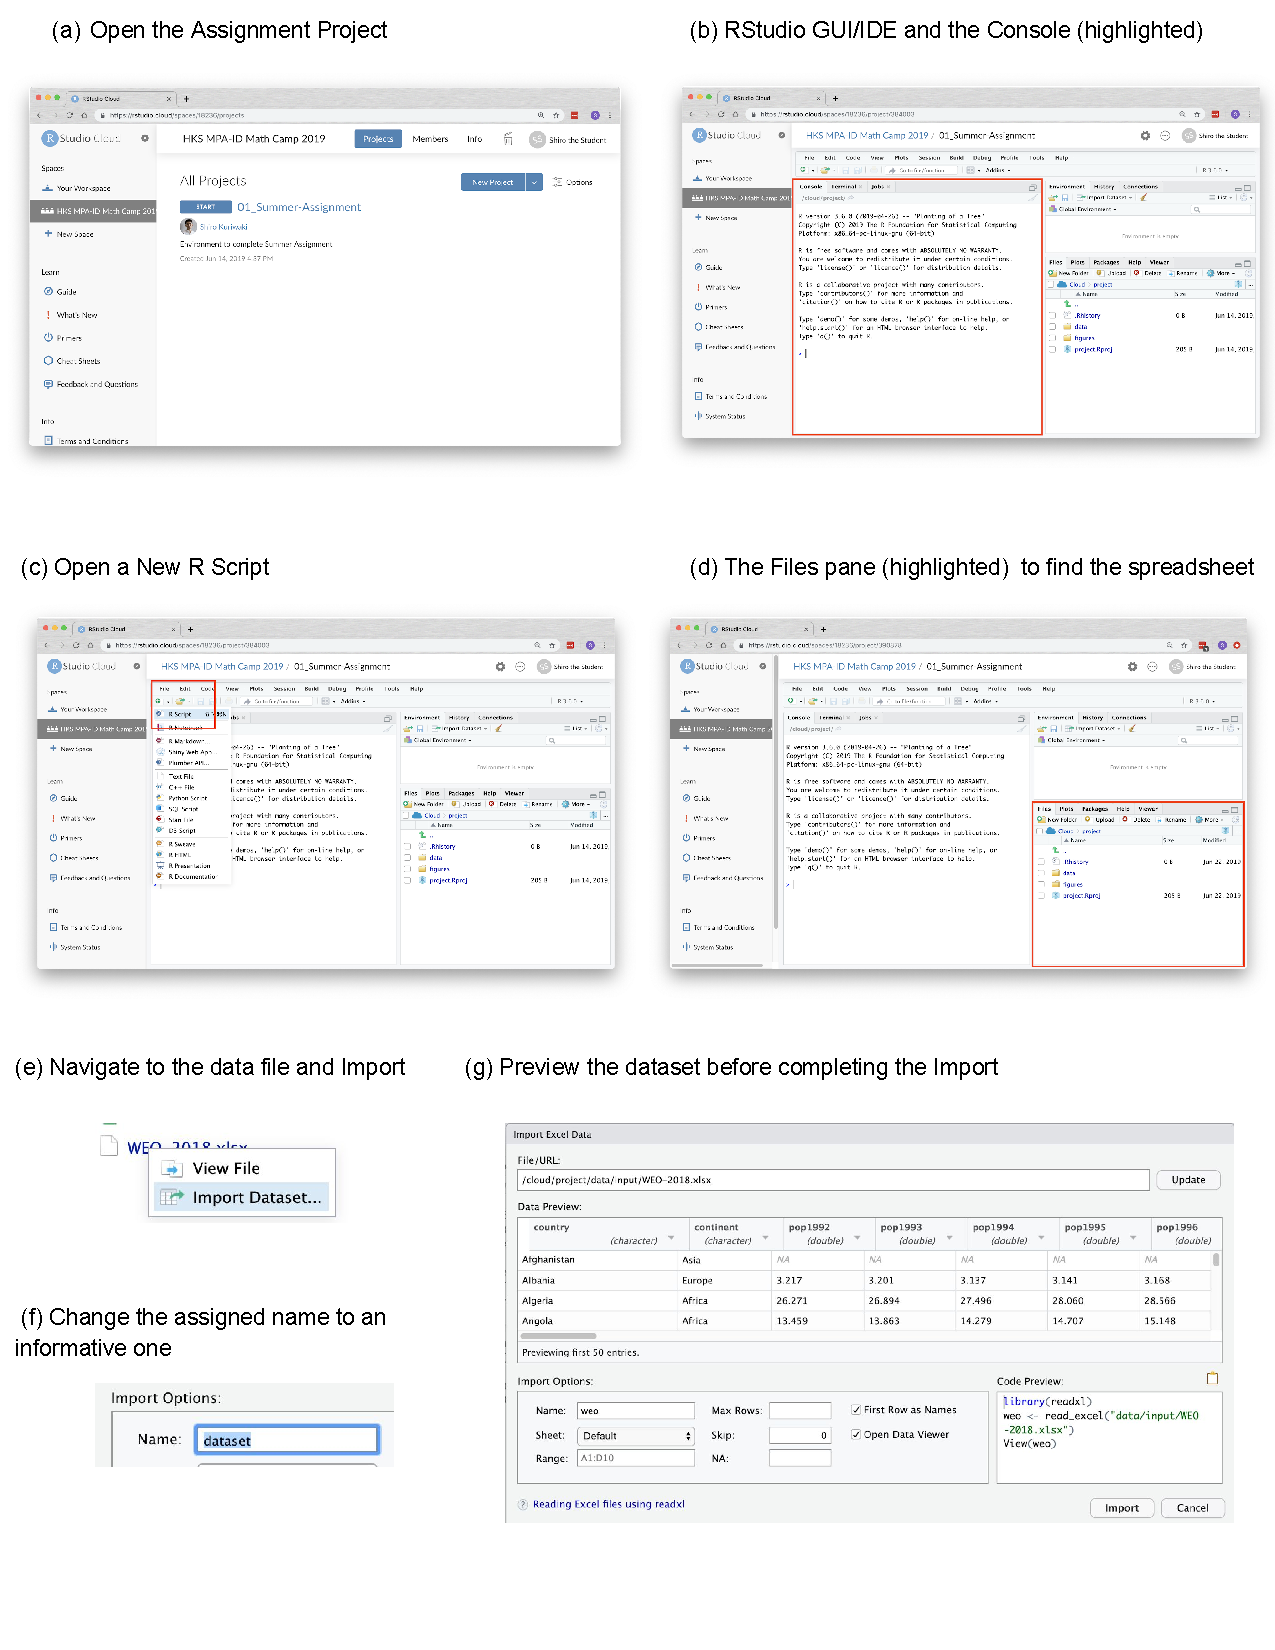
\includegraphics[width = \textwidth]{images/2019-06-17_assignment_images}
\caption{Example Screenshots Corresponding to Problem 2}
\end{figure}

\newpage

\hypertarget{problem-3-sorting-by-values}{%
\section*{Problem 3: Sorting by
Values}\label{problem-3-sorting-by-values}}
\addcontentsline{toc}{section}{Problem 3: Sorting by Values}

The following questions are based on a recent version of the World
Economic Outlook dataset published by the International Monetary Fund
(IMF), which you just read in. Each row in the spreadsheet is a country,
with total GDP for a given year adjusted for purchasing power parity
(with the \texttt{rgdp} column prefix) and total population (with the
\texttt{pop} column prefix). GDP values are in millions of 2011
international dollars, so you can directly compare values in different
years. Population values are in millions of persons.

\paragraph{(1)}

Write a command (connected by pipes) that (i) first sorts the dataset
from lowest to highest real GDP in 2017, and then (ii) outputs a
two-column dataset of the country and its GDP.

\begin{Shaded}
\begin{Highlighting}[]
\NormalTok{weo }\SpecialCharTok{\%\textgreater{}\%}
  \FunctionTok{arrange}\NormalTok{(rgdp2017) }\SpecialCharTok{\%\textgreater{}\%}
  \FunctionTok{select}\NormalTok{(country, rgdp2017)}
\end{Highlighting}
\end{Shaded}

\begin{verbatim}
## # A tibble: 191 x 2
##    country               rgdp2017
##    <chr>                    <dbl>
##  1 Tuvalu                    38.1
##  2 Nauru                    142. 
##  3 Marshall Islands         172. 
##  4 Kiribati                 207. 
##  5 Palau                    261. 
##  6 Micronesia               315. 
##  7 Tonga                    536. 
##  8 São Tomé and Príncipe    617. 
##  9 Vanuatu                  701. 
## 10 Dominica                 718. 
## # ... with 181 more rows
\end{verbatim}

\paragraph{(2)}

Write a command that is the same as (1) but now sorts it in descending
order of 2017 GDP (highest to lowest).

\begin{Shaded}
\begin{Highlighting}[]
\NormalTok{weo }\SpecialCharTok{\%\textgreater{}\%}
  \FunctionTok{arrange}\NormalTok{(}\FunctionTok{desc}\NormalTok{(rgdp2017)) }\SpecialCharTok{\%\textgreater{}\%}
  \FunctionTok{select}\NormalTok{(country, rgdp2017)}
\end{Highlighting}
\end{Shaded}

\begin{verbatim}
## # A tibble: 191 x 2
##    country         rgdp2017
##    <chr>              <dbl>
##  1 China          21094859.
##  2 United States  17662233.
##  3 India           8615891.
##  4 Japan           4944922.
##  5 Germany         3799057.
##  6 Russia          3650599.
##  7 Indonesia       2953727.
##  8 Brazil          2951498.
##  9 United Kingdom  2654284.
## 10 France          2582983.
## # ... with 181 more rows
\end{verbatim}

\paragraph{(3)}

The \code{arrange()} command can sort on more than one variable. To rank
countries within their continent, write a command that sorts the
countries by continent (in alphabetical order), then by 2017 GDP in
descending order. Remember different inputs (``arguments'') to a
function are separated by commas.

\begin{Shaded}
\begin{Highlighting}[]
\NormalTok{weo }\SpecialCharTok{\%\textgreater{}\%}
  \FunctionTok{arrange}\NormalTok{(continent, }\FunctionTok{desc}\NormalTok{(rgdp2017)) }\SpecialCharTok{\%\textgreater{}\%}
  \FunctionTok{select}\NormalTok{(continent, country, rgdp2017)}
\end{Highlighting}
\end{Shaded}

\begin{verbatim}
## # A tibble: 191 x 3
##    continent country      rgdp2017
##    <chr>     <chr>           <dbl>
##  1 Africa    Egypt        1094122.
##  2 Africa    Nigeria      1019039.
##  3 Africa    South Africa  697330.
##  4 Africa    Algeria       576494.
##  5 Africa    Morocco       271959.
##  6 Africa    Ethiopia      182365.
##  7 Africa    Angola        173327.
##  8 Africa    Sudan         170360.
##  9 Africa    Kenya         148596.
## 10 Africa    Tanzania      147711.
## # ... with 181 more rows
\end{verbatim}

\paragraph{(4)}

Write a command that shows African countries in descending order of
their 2017 GDP (Use the variable \texttt{continent} to filter on African
countries).

\begin{Shaded}
\begin{Highlighting}[]
\NormalTok{weo }\SpecialCharTok{\%\textgreater{}\%}
  \FunctionTok{filter}\NormalTok{(continent }\SpecialCharTok{==} \StringTok{"Africa"}\NormalTok{) }\SpecialCharTok{\%\textgreater{}\%}
  \FunctionTok{arrange}\NormalTok{(}\FunctionTok{desc}\NormalTok{(rgdp2017)) }\SpecialCharTok{\%\textgreater{}\%}
  \FunctionTok{select}\NormalTok{(country, rgdp2017)}
\end{Highlighting}
\end{Shaded}

\begin{verbatim}
## # A tibble: 55 x 2
##    country      rgdp2017
##    <chr>           <dbl>
##  1 Egypt        1094122.
##  2 Nigeria      1019039.
##  3 South Africa  697330.
##  4 Algeria       576494.
##  5 Morocco       271959.
##  6 Ethiopia      182365.
##  7 Angola        173327.
##  8 Sudan         170360.
##  9 Kenya         148596.
## 10 Tanzania      147711.
## # ... with 45 more rows
\end{verbatim}

\hypertarget{problem-4-gdp-per-capita}{%
\section*{Problem 4: GDP per capita}\label{problem-4-gdp-per-capita}}
\addcontentsline{toc}{section}{Problem 4: GDP per capita}

Create a new tibble object called \texttt{weo\_percap} that is the same
as the main dataset but also includes:

\begin{itemize}
\tightlist
\item
  A variable called \texttt{gdp\_percap\_2017} that is the country's GDP
  per capita in 2017,
\item
  A variable called \texttt{gdp\_percap\_1992}, which is the same as
  above but for 1992, and
\item
  A variable called \texttt{growth\_2017\_1992} which indicates the rate
  of growth between the two variables above, following the definition
  below.
\end{itemize}

Operationalize the rate of growth between two periods \(a\) and \(b >a\)
as:
\[\text{growth}_{b, a} = \frac{\text{GDP per capita}_b - \text{GDP per capita}_a}{\text{GDP per capita}_a}\]

\begin{Shaded}
\begin{Highlighting}[]
\NormalTok{weo\_percap }\OtherTok{\textless{}{-}}\NormalTok{ weo }\SpecialCharTok{\%\textgreater{}\%}
  \FunctionTok{mutate}\NormalTok{(}\AttributeTok{gdp\_percap\_2017 =}\NormalTok{ rgdp2017 }\SpecialCharTok{/}\NormalTok{ pop2017,}
         \AttributeTok{gdp\_percap\_1992 =}\NormalTok{ rgdp1992 }\SpecialCharTok{/}\NormalTok{ pop1992,}
         \AttributeTok{growth\_2017\_1992 =}\NormalTok{ gdp\_percap\_2017 }\SpecialCharTok{{-}}\NormalTok{ gdp\_percap\_1992)}
\end{Highlighting}
\end{Shaded}

You will be using this new object for the subsequent problems.

\hypertarget{problem-5-graphing}{%
\section*{Problem 5: Graphing}\label{problem-5-graphing}}
\addcontentsline{toc}{section}{Problem 5: Graphing}

\paragraph{(1)}

Make a scatterplot that shows a countries 1992 GDP per capita on the
x-axis and its 2017 GDP per capita on the
y-axis.\footnote{You might notice that the scatterplot itself is not as informative as it could be. In later sessions, we will spend time discussing the nuts and bolts of making a high-quality graphic that is informative and user-friendly.}

\begin{Shaded}
\begin{Highlighting}[]
\FunctionTok{ggplot}\NormalTok{(weo\_percap, }\FunctionTok{aes}\NormalTok{(gdp\_percap\_1992, gdp\_percap\_2017)) }\SpecialCharTok{+}
  \FunctionTok{geom\_point}\NormalTok{()}
\end{Highlighting}
\end{Shaded}

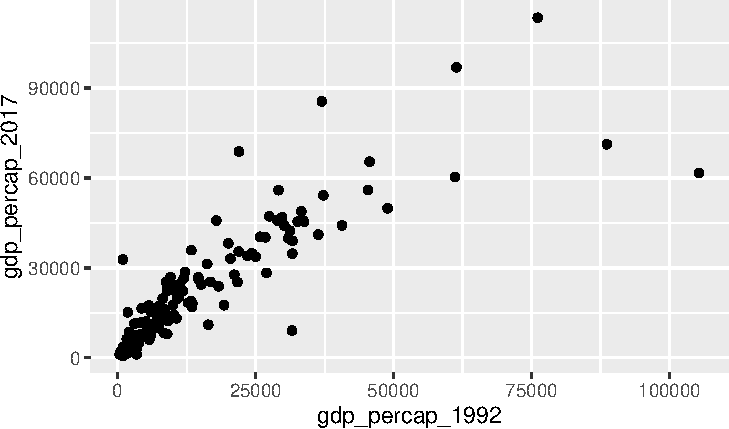
\includegraphics{pre-assignment_files/figure-latex/unnamed-chunk-7-1.pdf}

\paragraph{(2)}

Show the same figure, but coloring the points by continent. That is,
countries of the same continent should have the same color.

\begin{Shaded}
\begin{Highlighting}[]
\FunctionTok{ggplot}\NormalTok{(weo\_percap,}
       \FunctionTok{aes}\NormalTok{(}\AttributeTok{x =}\NormalTok{ gdp\_percap\_1992, }\AttributeTok{y =}\NormalTok{ gdp\_percap\_2017, }\AttributeTok{color =}\NormalTok{ continent)) }\SpecialCharTok{+}
  \FunctionTok{geom\_point}\NormalTok{()}
\end{Highlighting}
\end{Shaded}

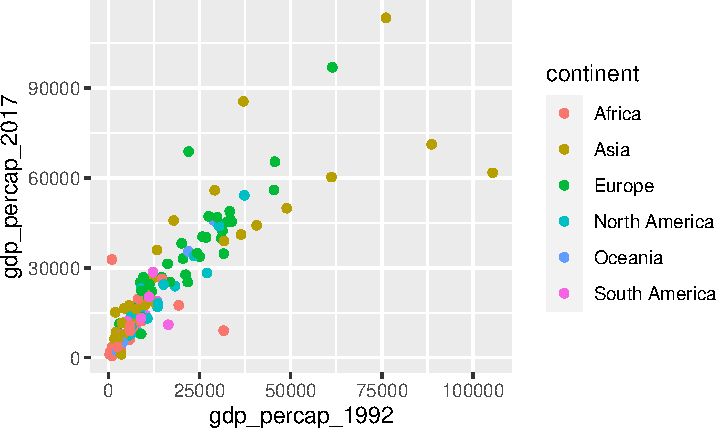
\includegraphics{pre-assignment_files/figure-latex/unnamed-chunk-8-1.pdf}

\paragraph{(3)}

Show the same figure, but assigning a different shape of point for
different continents. Also, set the color for all countries to navy by
using the color name \texttt{"navy"}.

\begin{Shaded}
\begin{Highlighting}[]
\FunctionTok{ggplot}\NormalTok{(weo\_percap,}
       \FunctionTok{aes}\NormalTok{(}\AttributeTok{x =}\NormalTok{ gdp\_percap\_1992, }\AttributeTok{y =}\NormalTok{ gdp\_percap\_2017, }\AttributeTok{shape =}\NormalTok{ continent)) }\SpecialCharTok{+}
  \FunctionTok{geom\_point}\NormalTok{(}\AttributeTok{color =} \StringTok{"navy"}\NormalTok{)}
\end{Highlighting}
\end{Shaded}

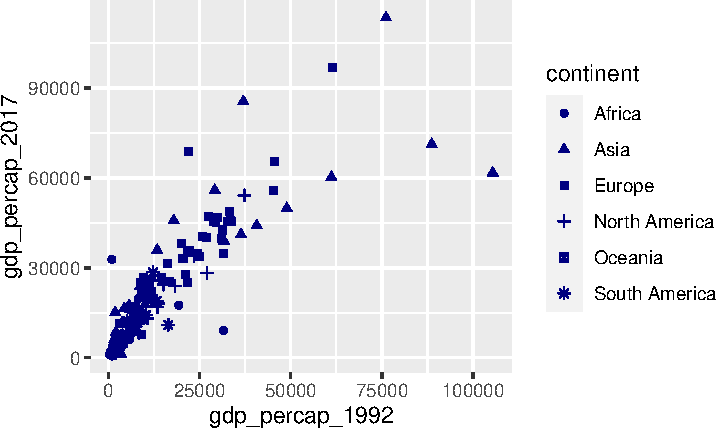
\includegraphics{pre-assignment_files/figure-latex/unnamed-chunk-9-1.pdf}

\paragraph{(4)}

To make a figure presentable in a professional setting, you will need to
many, many more additions to a graph. At the very least, you need to
label your axes with actual words. Update the graph in part (2) by
adding an informative x-axis title and a y-axis title. This can be
specified by adding a \texttt{labs()} layer to your graph. For an
example, open the help page for the \texttt{labs} function, and scroll
to the bottom of the page under ``Examples''.

\begin{Shaded}
\begin{Highlighting}[]
\FunctionTok{ggplot}\NormalTok{(weo\_percap, }\FunctionTok{aes}\NormalTok{(}\AttributeTok{x =}\NormalTok{ gdp\_percap\_1992, }
                       \AttributeTok{y =}\NormalTok{ gdp\_percap\_2017, }
                       \AttributeTok{color =}\NormalTok{ continent)) }\SpecialCharTok{+}
  \FunctionTok{geom\_point}\NormalTok{() }\SpecialCharTok{+}
  \FunctionTok{labs}\NormalTok{(}\AttributeTok{x =} \StringTok{"GDP per capita in 1992"}\NormalTok{,}
       \AttributeTok{y =} \StringTok{"GDP per capita in 2007"}\NormalTok{,}
       \AttributeTok{color =} \StringTok{"Continent"}\NormalTok{)}
\end{Highlighting}
\end{Shaded}

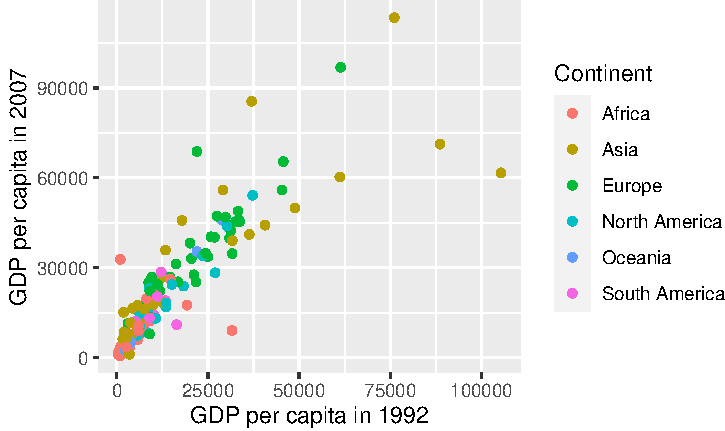
\includegraphics{pre-assignment_files/figure-latex/unnamed-chunk-10-1.pdf}

\hypertarget{problem-6-mean-and-median}{%
\section*{Problem 6: Mean and Median}\label{problem-6-mean-and-median}}
\addcontentsline{toc}{section}{Problem 6: Mean and Median}

\paragraph{(1)}

Let's start to think about summarizing variables using summary
statistics. Write code that reports the mean of country-level GDP per
capita of 2017 in one column and the median for 2017 in another. Pick
column names that are sufficiently self-explanatory but also concise.

\begin{Shaded}
\begin{Highlighting}[]
\NormalTok{weo\_percap }\SpecialCharTok{\%\textgreater{}\%}
  \FunctionTok{summarize}\NormalTok{(}\AttributeTok{mean\_gcap\_2017 =} \FunctionTok{mean}\NormalTok{(gdp\_percap\_2017),}
            \AttributeTok{median\_gcap\_2017 =} \FunctionTok{median}\NormalTok{(gdp\_percap\_2017))}
\end{Highlighting}
\end{Shaded}

\begin{verbatim}
## # A tibble: 1 x 2
##   mean_gcap_2017 median_gcap_2017
##            <dbl>            <dbl>
## 1         18915.           11590.
\end{verbatim}

\paragraph{(2)}

Write code that indicates which countries have missing values for 1992
GDP per capita and 2017 GDP per capita.

\begin{Shaded}
\begin{Highlighting}[]
\NormalTok{weo\_percap }\SpecialCharTok{\%\textgreater{}\%}
  \FunctionTok{filter}\NormalTok{(}\FunctionTok{is.na}\NormalTok{(gdp\_percap\_1992)) }\SpecialCharTok{\%\textgreater{}\%}
  \FunctionTok{select}\NormalTok{(country)}
\end{Highlighting}
\end{Shaded}

\begin{verbatim}
## # A tibble: 25 x 1
##    country               
##    <chr>                 
##  1 Afghanistan           
##  2 Bosnia and Herzegovina
##  3 Czech Republic        
##  4 Estonia               
##  5 Georgia               
##  6 Iraq                  
##  7 Kosovo                
##  8 Liberia               
##  9 Lithuania             
## 10 Macao                 
## # ... with 15 more rows
\end{verbatim}

\begin{Shaded}
\begin{Highlighting}[]
\NormalTok{weo\_percap }\SpecialCharTok{\%\textgreater{}\%}
  \FunctionTok{filter}\NormalTok{(}\FunctionTok{is.na}\NormalTok{(gdp\_percap\_2017)) }\SpecialCharTok{\%\textgreater{}\%}
  \FunctionTok{select}\NormalTok{(country)}
\end{Highlighting}
\end{Shaded}

\begin{verbatim}
## # A tibble: 0 x 1
## # ... with 1 variable: country <chr>
\end{verbatim}

\paragraph{(3)}

Try the same as (1) but now with replacing 2017 with 1992. You should
initially notice that you get a missing value for both summary
statistics. This is because by default, \code{mean()} and
\code{median()} report a missing value if at least one of its input
values is missing, and as you probably found in part (2), some countries
have have missing values for 1992 GDP per capita. Now, modify your code
so that you change this default and ignore the missing values in your
computation. As the help page for the functions indicate, the relevant
argument is \code{na.rm} (for NA - remove). Change its logical value
from \code{FALSE} (its default) to \code{TRUE}, while making sure to
follow the style guide for proper spacing (style guide section 2.2.3).

\begin{Shaded}
\begin{Highlighting}[]
\NormalTok{weo\_percap }\SpecialCharTok{\%\textgreater{}\%}
  \FunctionTok{summarize}\NormalTok{(}\AttributeTok{mean\_gcap\_1992 =} \FunctionTok{mean}\NormalTok{(gdp\_percap\_1992, }\AttributeTok{na.rm =} \ConstantTok{TRUE}\NormalTok{),}
            \AttributeTok{median\_gcap\_1992 =} \FunctionTok{median}\NormalTok{(gdp\_percap\_1992, }\AttributeTok{na.rm =} \ConstantTok{TRUE}\NormalTok{))}
\end{Highlighting}
\end{Shaded}

\begin{verbatim}
## # A tibble: 1 x 2
##   mean_gcap_1992 median_gcap_1992
##            <dbl>            <dbl>
## 1         12894.            6819.
\end{verbatim}

\hypertarget{problem-7-slice-and-filter}{%
\section*{Problem 7: slice() and
filter()}\label{problem-7-slice-and-filter}}
\addcontentsline{toc}{section}{Problem 7: slice() and filter()}

Much of data analysis is understanding how new functions work through
reading the documentation and experimentation. The function
\code{slice()} is part of the tidyverse and allows you to filter rows by
their position. Notice that \code{slice()} and \code{filter()} are
similar in that they subset rows of a dataset, but differ in the types
of input they require --- the former asks for positions, the latter asks
for conditions.

Check out the help page of \code{slice()} (recall, e.g., by typing
\code{?slice} in the Console). Then, write a command that shows the
countries with the top three and bottom three 2017 GDPs, thereby
combining the output in the first two R exercises.

\begin{Shaded}
\begin{Highlighting}[]
\NormalTok{weo }\SpecialCharTok{\%\textgreater{}\%}
 \FunctionTok{arrange}\NormalTok{(}\FunctionTok{desc}\NormalTok{(rgdp2017)) }\SpecialCharTok{\%\textgreater{}\%}
 \FunctionTok{select}\NormalTok{(country, rgdp2017) }\SpecialCharTok{\%\textgreater{}\%}
 \FunctionTok{slice}\NormalTok{(}\FunctionTok{c}\NormalTok{(}\DecValTok{1}\SpecialCharTok{:}\DecValTok{3}\NormalTok{, }\DecValTok{189}\SpecialCharTok{:}\DecValTok{191}\NormalTok{))}
\end{Highlighting}
\end{Shaded}

\begin{verbatim}
## # A tibble: 6 x 2
##   country            rgdp2017
##   <chr>                 <dbl>
## 1 China            21094859. 
## 2 United States    17662233. 
## 3 India             8615891. 
## 4 Marshall Islands      172. 
## 5 Nauru                 142. 
## 6 Tuvalu                 38.1
\end{verbatim}

\hypertarget{optional-and-challenging-more-graphing}{%
\section*{{[}Optional and Challenging{]} More
Graphing}\label{optional-and-challenging-more-graphing}}
\addcontentsline{toc}{section}{{[}Optional and Challenging{]} More
Graphing}

\emph{Note}: This problem is optional; it involves some commands not
covered in the primers.

\medskip

Make a graph like the one shown in Figure \ref{fig:hard_scatter}. Follow
both the graphical components of the graph shown as you see them, as
well as the description of the measures as described in the Figure
caption. \emph{Hint:} Check out the packages \code{ggrepel} and
\code{scales} to implement some of the features.

\begin{Shaded}
\begin{Highlighting}[]
\CommentTok{\# only use large enough countiries}
\NormalTok{ds\_large }\OtherTok{\textless{}{-}}\NormalTok{ weo\_percap }\SpecialCharTok{\%\textgreater{}\%}
  \FunctionTok{filter}\NormalTok{(pop1992 }\SpecialCharTok{\textgreater{}} \DecValTok{5} \SpecialCharTok{|}\NormalTok{ pop2017 }\SpecialCharTok{\textgreater{}} \DecValTok{5}\NormalTok{)}

\CommentTok{\# subset to show country names. Only use the top 5.}
\NormalTok{sub\_show }\OtherTok{\textless{}{-}}\NormalTok{ ds\_large }\SpecialCharTok{\%\textgreater{}\%}
  \FunctionTok{mutate}\NormalTok{(}\AttributeTok{abs\_change =} \FunctionTok{abs}\NormalTok{(gdp\_percap\_2017 }\SpecialCharTok{{-}}\NormalTok{ gdp\_percap\_1992)) }\SpecialCharTok{\%\textgreater{}\%}
  \FunctionTok{arrange}\NormalTok{(}\FunctionTok{desc}\NormalTok{(abs\_change)) }\SpecialCharTok{\%\textgreater{}\%}
  \FunctionTok{select}\NormalTok{(country, gdp\_percap\_2017, gdp\_percap\_1992) }\SpecialCharTok{\%\textgreater{}\%}
  \FunctionTok{slice}\NormalTok{(}\DecValTok{1}\SpecialCharTok{:}\DecValTok{5}\NormalTok{)}

\CommentTok{\# Creat the graph, but add a layer of geom\_text\_repel and input the subset there }
\NormalTok{gg\_scatter }\OtherTok{\textless{}{-}} \FunctionTok{ggplot}\NormalTok{(ds\_large, }\FunctionTok{aes}\NormalTok{(gdp\_percap\_1992, gdp\_percap\_2017)) }\SpecialCharTok{+}
  \FunctionTok{geom\_abline}\NormalTok{(}\AttributeTok{intercept =} \DecValTok{0}\NormalTok{, }\AttributeTok{slope =} \DecValTok{1}\NormalTok{, }\AttributeTok{linetype =} \StringTok{"dashed"}\NormalTok{) }\SpecialCharTok{+}
  \FunctionTok{geom\_point}\NormalTok{(}\FunctionTok{aes}\NormalTok{(}\AttributeTok{size =}\NormalTok{ pop2017), }\AttributeTok{alpha =} \FloatTok{0.5}\NormalTok{) }\SpecialCharTok{+}
  \FunctionTok{coord\_equal}\NormalTok{() }\SpecialCharTok{+}
  \FunctionTok{geom\_text\_repel}\NormalTok{(}\AttributeTok{data =}\NormalTok{ sub\_show, }\FunctionTok{aes}\NormalTok{(}\AttributeTok{label =}\NormalTok{ country)) }\SpecialCharTok{+}
  \FunctionTok{scale\_x\_continuous}\NormalTok{(}\AttributeTok{labels =}\NormalTok{ dollar) }\SpecialCharTok{+}
  \FunctionTok{scale\_y\_continuous}\NormalTok{(}\AttributeTok{labels =}\NormalTok{ dollar) }\SpecialCharTok{+}
  \FunctionTok{guides}\NormalTok{(}\AttributeTok{size =} \ConstantTok{FALSE}\NormalTok{) }\SpecialCharTok{+}
  \FunctionTok{labs}\NormalTok{(}\AttributeTok{x =} \StringTok{"1992 GDP per Capita"}\NormalTok{,}
       \AttributeTok{y =} \StringTok{"2017 GDP per Capita"}\NormalTok{,}
       \AttributeTok{caption =} \StringTok{"Points sized by 2017 population and labels show top 5 countries}
\StringTok{       with the most absolute change. Only countries with population at least 5 million}\SpecialCharTok{\textbackslash{}n}\StringTok{in 1992 or 2017 shown. Dotted line indicates 45{-}degree line."}\NormalTok{)}

\FunctionTok{ggsave}\NormalTok{(}\StringTok{"gg\_scatter.pdf"}\NormalTok{, gg\_scatter, }\AttributeTok{width =} \DecValTok{5}\NormalTok{, }\AttributeTok{height =} \DecValTok{5}\NormalTok{)}
\end{Highlighting}
\end{Shaded}

\begin{figure}[!h]
\centering
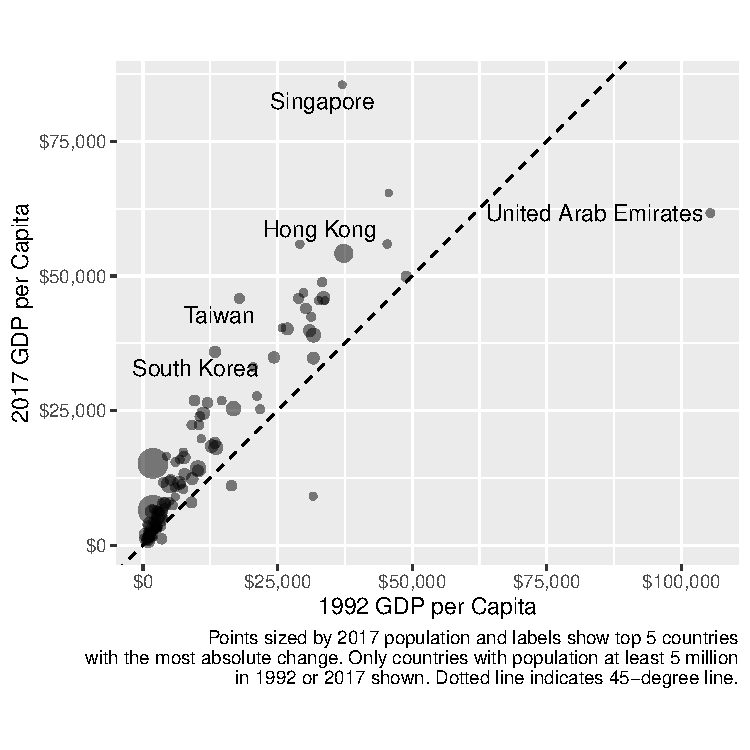
\includegraphics[width = 0.9\linewidth]{images/gg_scatter.pdf}
\caption{Changes in GDP per capita between 1992 and 2017.}
\label{fig:hard_scatter}
\end{figure}

\newpage

\hypertarget{submitting-and-survey}{%
\section*{Submitting (and Survey)}\label{submitting-and-survey}}
\addcontentsline{toc}{section}{Submitting (and Survey)}

Before you submit, please complete this brief survey as so that we
understand better you background and can design the R activities in math
camp accordingly.

\bigskip

\url{https://harvard.az1.qualtrics.com/jfe/form/SV_0jLN9xCSLAWn2Ul}

\bigskip

Once you have completed or made an attempt for all the problem, please
clean up your R script, download it from the cloud, and submit it to
Canvas.

Math camp instructors will check and provide comments for your code. You
should follow these guidelines to clean up your final submission (and
should do so for all future scripts):

\begin{itemize}
\tightlist
\item
  Delete any failed attempts or duplicative code.
\item
  Label the relevant question number by comment (e.g.,
  \code{\#\# Problem 1.1 -------}. Follow the style guide for the exact
  format).
\item
  You do not need to submit anything other than the R script (i.e.,
  figures or numbers not necessary), but the results should be
  ``reproducible'' from the script. This means that an instructor who
  receives your script should be able to run it and reproduce correct
  answers. To preview this, try restarting R (Toolbar \texttt{Session}
  \textgreater{} \texttt{Restart}) and running your entire code at once
  (e.g., Select All Text and Run, or \texttt{Run\ All} by the hot-key
  \texttt{option} + \texttt{command} + \texttt{R}. Before you do this,
  though, make sure you explicitly load the \texttt{tidyverse} package
  in your code by adding \code{library(tidyverse)} to the beginning of
  your file.
\item
  Follow other guidelines from the style guide, such as breaking up long
  lines and properly using spaces.
\item
  As we mentioned in the beginning, please name your script with your
  last name followed by your first name, all in lower case. This helps
  graders sort through all submissions.
\end{itemize}

After editing your code, save it to the main project folder, and then
download it by right-clicking the file icon (in the Files pane), and
selecting \texttt{Export} (Figure \ref{fig:export}). Download the script
and attach it to your Canvas submission.

\FloatBarrier

\begin{figure}[!h]
\centering
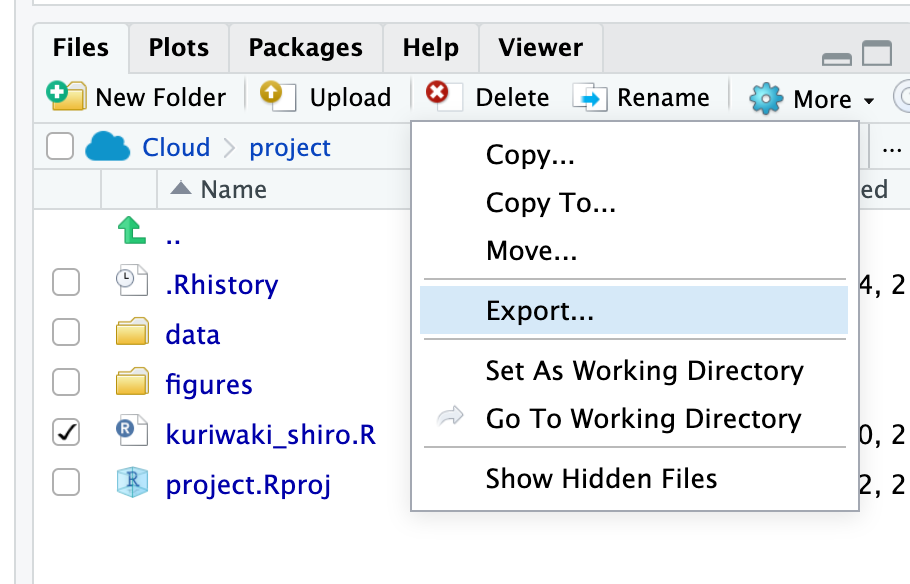
\includegraphics[width = 0.5\linewidth]{images/07_export.png}
\caption{Downloading your final script}
\label{fig:export}
\end{figure}
\end{document}



